\documentclass[table]{beamer}
\usetheme{Boadilla}

\usepackage[utf8]{inputenc}
\usepackage[full]{textcomp}
\usepackage[T1]{fontenc}
\usepackage{graphicx}
\usepackage{algorithm,algpseudocode}
\usepackage{color}
\usepackage{tikz,pgf}
\usetikzlibrary{matrix,shapes,arrows,shadows,calc,decorations.markings,fit}
\usepackage{amsmath, amsthm, amssymb}
\usepackage{url}
\usepackage{hyperref}
\usepackage{comment}
%\beamertemplatenavigationsymbolsempty

\providecommand{\jlcm}{\mbox{\textit{j}LCM} }
\providecommand{\toppi}{\mbox{\textsc{TopPI}} }
\providecommand{\capa}{\mbox{\textsc{CAPA}} }
\providecommand{\datalyse}{\mbox{\textsc{Datalyse}} }

\providecommand{\nbm}{39 {}}

\providecommand{\demoassoc}{\texttt{demo\-\_assoc} }
\providecommand{\prodassocreceipt}{\texttt{prod\-\_assoc\-\_receipt} }
\providecommand{\prodassocclient}{\texttt{prod\-\_assoc\-\_client} }


\title[PhD defense]{Mining and ranking closed itemsets from large-scale transactional datasets}
\author[M. Kirchgessner]{Martin Kirchgessner}
\institute[LIG]{
  Laboratoire d'Informatique de Grenoble\\
	\texttt{martin.kirchgessner@imag.fr}
}
\date[September 26, 2016]{September 26, 2016}

\begin{document}

\begin{frame}[plain]
	\titlepage
\end{frame}

\begin{frame}{Outline}
  \tableofcontents
\end{frame}




\section{Data of interest}


\begin{frame}{Over year 2013 at Intermarché}
One of the major food stores in France
\begin{itemize}
  %\tightlist
  \item 9,267,961 customers
  \item 290,734,163 tickets
  \item 222,228 different products
\end{itemize}
\end{frame}

\begin{frame}[t]{Additional data}
  \begin{figure}
    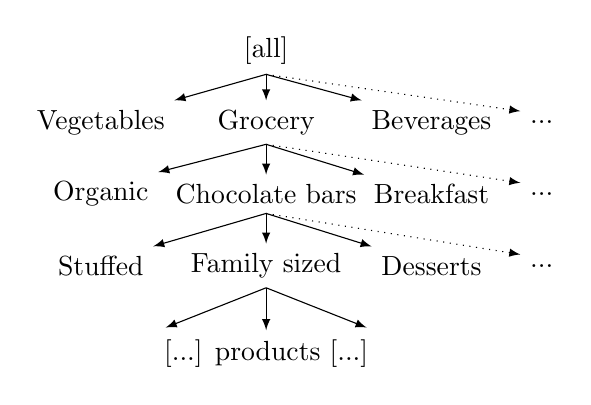
\begin{tikzpicture}[>=latex,scale=0.7]
      \tikzstyle{every node}=[font=\Tiny]
      
\node (root) at (-1,0) {[all]};

\node (A_farleft) at (-4, -1.3) {Vegetables};
\draw [->] (root.south) -- (A_farleft.north east);

\node (A_left) at (-1,-1.3) {Grocery};
\draw [->] (root.south) -- (A_left.north);

\node (A_right) at (2,-1.3) {Beverages};
\draw [->] (root.south) -- (A_right.north west);

\node (A_farright) at (4,-1.3) {...};
\draw [->,dotted] (root.south) -- (A_farright.north west);

\node (B_farleft) at (-4,-2.6) {Organic};
\draw [->] (A_left.south) -- (B_farleft.north east);

\node (B_left) at (-1, -2.6) {Chocolate bars};
\draw [->] (A_left.south) -- (B_left.north);

\node (B_right) at (2, -2.6) {Breakfast};
\draw [->] (A_left.south) -- (B_right.north west);

\node (B_farright) at (4, -2.6) {...};
\draw [->,dotted] (A_left.south) -- (B_farright.north west);

\node (C_farleft) at (-4, -3.9) {Stuffed};
\draw [->] (B_left.south) -- (C_farleft.north east);

\node (C_left) at (-1, -3.9) {Family sized};
\draw [->] (B_left.south) -- (C_left.north);

\node (C_right) at (2, -3.9) {Desserts};
\draw [->] (B_left.south) -- (C_right.north west);

\node (C_farright) at (4, -3.9) {...};
\draw [->, dotted] (B_left.south) -- (C_farright.north west);

\node (D_l) at (-3, -5.2) {};
\draw [->] (C_left.south) -- (D_l.north east);
\node (D) at (-1, -5.5) {[...] products [...] };
\draw [->] (C_left.south) -- (D.north);
\node (D_r) at (1, -5.2) {};
\draw [->] (C_left.south) -- (D_r.north west);

    \end{tikzpicture}
    \includegraphics[width=0.45\textwidth]{fig/departements.pdf}
  \end{figure}
\end{frame}


\begin{frame}{Our complete model}
  \begin{figure}
    \includegraphics[width=\textwidth]{../tikz/input_model_standalone}
  \end{figure}
\end{frame}



\begin{frame}{Items distribution in our experimental datasets.}
  \begin{center}
    \includegraphics[width=\linewidth]{../fig/itemFreqCumulativeDist/itemFreqCumulativeDistributions.pdf}
  \end{center}
\end{frame}


\begin{frame}{Interesting trends - 3 scenarios}
  Final users: central marketing analysts.\\
  \begin{itemize}
    \item \demoassoc \\
      {\em  Women below 35 y.o. tend to buy baby food}\\
      {\em  People from the {\em Nord} department tend to buy sodas}
    \item \prodassocclient: per-client products associations \\
      People who ever baught {\em vanilla cream} also bought {\em chocolate cream}
    \item \prodassocreceipt: per-ticket products associations\\
      {\em Pork sausage} and {\em mustard} are often baught simultaneously with {\em dry Riesling}
\end{itemize}
\end{frame}

\begin{frame}{System overview}
  % trim={<left> <lower> <right> <upper>}
  \begin{figure}
    \only<1>{\includegraphics[clip]{../tikz/arch_standalone}}
    \only<2>{\includegraphics[trim={0 0 0 4cm},clip]{../tikz/arch_standalone}}
    \only<3>{\includegraphics[trim={2.5cm 0 0 8cm},clip]{../tikz/arch_standalone}}
    \only<4>{\includegraphics[trim={5cm 0 0 15cm},clip]{../tikz/arch_standalone}}
    \only<5>{\includegraphics[trim={0 0 0 15cm},clip]{../tikz/arch_standalone}}
  \end{figure}
\end{frame}

\begin{frame}{System overview}
  \begin{enumerate}
    \item Nightly tickets transfer to the central store
    \item Enrichment with taxonomy/demographics (HBase)
    \item Curating $\cal D$: mining scenarios and target definition\\
      \begin{itemize}
        \item Analyst may request any form of association rule
        \item Over any set of target products/categories/populations
      \end{itemize}
    \item Association rules mining
    \item Rules ranking and exploration

    TODO: pause and highlight Mining and Ranking
  \end{enumerate}
\end{frame}

\begin{frame}{Transactional datasets}
  \begin{block}{Input}
    Given ${\cal I}$, a set of items.\\
    A collection ${\cal D}$ of {\em transactions} $\langle t_1,...,t_n\rangle$,
    where each $t_j \subseteq {\cal I}$.
  \end{block}
  \pause
  \begin{block}{Output (presented to the analyst)}
    A collection of {\em closed} itemsets (CIS),\\
    {\em ie.} itemsets $P$ satisfying
    $\nexists Q \supset P$ s.t. $\mathit{support}_{\cal D}(P) = \mathit{support}_{\cal D}(Q)$.
  \end{block}
  Where $\mathit{support}_{\cal D}(P) = |\{t \in {\cal D} | P \subset t\}|$.
  \vfill
	\begin{footnotesize}
    [12] {\em Discovering frequent closed itemsets for association rules}, \\
    Pasquier, Bastide, Taouil, Lakhal @ ICDT'99
	\end{footnotesize}
\end{frame}


\begin{frame}{Frequency-based item ordering}
  Internally, items are represented as integers, indexed by decreasing frequency:
  \begin{itemize}
    \item $0$ is the most frequent item
    \item $1$ the second most
    \item etc...
  \end{itemize}
\end{frame}


\begin{frame}{Examples: \prodassocreceipt}
  Items are products, transactions are customers' tickets.
  \\\vspace{1em}
  \begin{scriptsize}
  \begin{itemize}
    \item MOULIN. MODULE PETIT DEJEUNE, BALAI PVC 60CM SM
    \item BRANDADE MORUE 300G, MOISSON 6 OEUFS, HC240X220+2TO OCEAN, DH 140X190 OCEAN, TT 90X185 OCEAN
    \item CROQUET.ADULTE 10KG
    \item \ldots
  \end{itemize}
  \vspace{1em}
  \begin{table}
    \centering
    \def\arraystretch{1.2}
    \begin{tabular}{|c|c|c|}
      \hline
      $A \rightarrow B$       & $\mathit{support}(A)$ & $\mathit{support}(A \cup B)$ \\\hline
      LIEGEOIS CHOCO 4X100G $\rightarrow$  CR.DESS.CHOCO 4X115G       & $477,710$ & $98,693$   \\
      \{P.FEUILLT ROULE, PREP.FRANGIPANE\}    &                 &     \\
          $\rightarrow$ SUCRE POUDRE 1/2KG & $9,743$ & $522$  \\
      \hline
    \end{tabular}
  \end{table}
  \end{scriptsize}
\end{frame}

\begin{frame}[t]{Examples: \demoassoc}
  Items are product categories and demographic attributes.\\
  A transaction is a customer's demographics and purchased products' categories.\\\vspace{1em}
  \begin{scriptsize}
    \begin{itemize}
      \item {\em <35, Male, Auvergne, Allier}, SURGELES, CRUSTACES, BISCUITS FRUITES, BALLADEUR AUDIO,
        PETITE PUERICULTURE, D.P.H., MOUCHOIR \& PH, ... \\
      \item {\em <35, Female, Rhône-Alpes, Isère}, FRUITS ET LEGUMES, F/L FRAIS EMBALLE, F/L REFRIGERE DLC COURTE,
        EPICERIE SALEE, FARINES, FARINE PREPA PAINS, ... \\
    \end{itemize}
    \begin{table}[t!]
      \def\arraystretch{1.2}
      \begin{tabular}{|c|c|c|}
        \hline
        $A \rightarrow B$       & $\mathit{support}(A)$ & $\mathit{support}(A \cup B)$ \\\hline
        {\em Alsace} $\rightarrow$ PAINS DE CAMPAGNE & 2,843,532 & 28,889  \\
        {\em 35-49, Female} $\rightarrow$  PRODUITS SOLAIRES  & 49,677,175 & 196,612   \\
        \hline
      \end{tabular}
    \end{table}
  \end{scriptsize}
  $A$ only includes demographic attributes,\\
  $B$ is always a single products category.
\end{frame}









\section{Mining item-centric top-k closed itemsets with \toppi}

\subsection{Item-Centric Mining?}

\begin{frame}
  Item-Centric Mining?
\end{frame}

\begin{frame}[t]{Big transactional datasets}
  ``big'' means our datasets contain at least
  \begin{itemize}
    \item Thousands/millions of items in $\cal I$
    \item Millions of transactions in $\cal D$
  \end{itemize}
  \pause
  \begin{center}
    \includegraphics[width=.5\linewidth]{fig/freq_distrib.pdf}
  \end{center}
  \begin{footnotesize}
    [2] {\em The Long Tail: Why the Future of Business Is Selling Less of More},
    \\ Anderson (2006)
  \end{footnotesize}
\end{frame}


\begin{frame}[t]{Frequent Itemset Mining on big datasets}
  \begin{center}
    \includegraphics[width=.5\linewidth]{fig/freq_distrib_standard.pdf}
  \end{center}
  \begin{itemize}
    \item Which minimum support yields interesting results?
    \pause
    \item Are all closed itemsets interesting?
    \pause
    \item What about the remaining items?
  \end{itemize}
\end{frame}


\begin{frame}[t]{Item-Centric Mining}
  \begin{center}
    \only<1>{\includegraphics[width=.5\linewidth]{fig/freq_distrib_standard.pdf}}
    \only<2->{\includegraphics[width=.5\linewidth]{fig/freq_distrib_toppi.pdf}}
  \end{center}
  \only<2>{
    Replace the minimum support by a single parameter, $k$
  }
\end{frame}

\begin{frame}{Item-Centric Mining}
  \begin{block}{\toppi's problem statement}
    Given a transactional dataset $\cal D$ and an integer $k$,\\
    return, $\forall i \in {\cal I}$, $\mathit{top}(i)$:
    the $k$ most frequent CIS containing $i$.
  \end{block}
  \vspace{1em}
  \toppi stands for ``Top {\bf P}er {\bf I}tem''.
  \vspace{1em}
  \pause
  \begin{block}{Benefits}
    \begin{itemize}
      \item Restrict intuitively the CIS space
      \pause
      \item Resulting collection is easy to browse
    \end{itemize}
  \end{block}
  \pause
  We target high-end, multi-core servers.
\end{frame}







\subsection{Related Work}

\begin{frame}{Related Work}
  Can we implement Item-Centric Mining using existing methods ?
\end{frame}

\begin{frame}{Our baseline: Item-Centric Mining with TFP}
  \vbox to .8\textheight{%
  \begin{block}{Implementation with a top-$k$ CIS miner, TFP}
    For each item $i$:
    \begin{itemize}
      \item Instantiate ${\cal D}[i]=\{t \in {\cal D} | i \in t\}$
      \item Launch TFP on ${\cal D}[i]$, yielding $\mathit{top}(i).$
    \end{itemize}
  \end{block}
  \only<2->{
    Easy to parallelize, fine for small files.
  }
  \only<3->{%
    \begin{alertblock}{Not sufficient for our datasets}
      Even with ad-hoc optimizations:
      \begin{itemize}
        \item Keep only top-k-frequent items in ${\cal D}[i]$
        \item Index transactions by item for an instant access to ${\cal D}[i]$.
      \end{itemize}
    \end{alertblock}
  }%
  \vfill
	\begin{footnotesize}
    [6] {\em Mining top-k frequent closed patterns without minimum support.}\\
    Han, Wang, Lu, Tzvetkov @ ICDM'02
	\end{footnotesize}
  }%
\end{frame}

\begin{frame}{PFP: parallel FP-Growth}
  \vbox to .8\textheight{%
  \begin{itemize}
    \item An algorithm for the MapReduce platform.
    \item Returns, $\forall i \in {\cal I}$, at most $k$ itemsets containing $i$.
    \only<2->{
    \item Implementation available in (old versions of) Mahout.
      \begin{itemize}
        \item Much more resource-consuming than \toppi and its baseline.
      \end{itemize}
    }
  \end{itemize}
  \vfill
	\begin{footnotesize}
    [9] {\em PFP: parallel FP-growth for query recommendation.}\\
    Li, Wang, Zhang, Zhang, Chang @ RecSys'08
	\end{footnotesize}
  }%
\end{frame}

\begin{frame}{Efficiently enumerating CIS}
  \vbox to .8\textheight{%
    \toppi has to find closed itemsets (CIS) and their support,
    \\but only those likely to appear in $\mathit{top}(i)$ for an item $i$.
    \vspace{1em}
    \only<2->{
    \\Enumeration is inspired from PLCM.\\
    }
    \vspace{1em}
    \only<3->{
      (P)LCM shapes the CIS lattice as a tree (depth-first traversal).
      \begin{block}{Tree property}
        In a branch, all itemsets $P$ have the same $\mathit{max}(P)$.
      \end{block}
    }
    \vfill
    \only<2->{
      \begin{footnotesize}
        [11] {\em  Discovering closed frequent itemsets on multi-core: Parallelizing computations and optimizing memory accesses.}\\
            Négrevergne, Termier, Méhaut, Uno @ HPCS'10
      \end{footnotesize}
    }
  }
\end{frame}

\begin{frame}{Frequency-based item ordering}
  \begin{itemize}
    \item $0$ is the most frequent item
    \item $1$ the second most
    \item etc...
  \end{itemize}
  \pause
  \vspace{1em}
  In a branch, an item is combined with items which are more frequent (globally).

  \vspace{1em}
  The $\mathit{top}(i)$ heaps are firstly filled for the most frequent items.
\end{frame}

\begin{comment}
                      \begin{frame}{Traversing the closed itemsets space}
                        \vbox to .8\textheight{%
                        Which algorithms family can we pick?
                        \begin{itemize}
                          \pause
                          \item Too many items for generate-and-test (APriori)
                          \only<3->{
                          \item A corner case for prefix trees
                            \begin{itemize}
                              \item $90$ to $99\%$ of transactions are unique.
                              \item Not cache-friendly when multi-threaded.
                            \end{itemize}
                          }
                        \end{itemize}
                        \only<4->{
                          Our CIS enumeration is akin to PLCM.
                        }
                        \pause
                        \only<5->{
                          \begin{alertblock}{Not sufficient for our datasets}
                            The support threshold is essential to these algorithms' performance.
                          \end{alertblock}
                        }

                        \vfill
                        \only<2>{
                      	\begin{footnotesize}
                          [1] {\em Fast algorithms for mining association rules in large databases},\\
                          Agrawal, Srikant @ VLDB'94
                      	\end{footnotesize}
                        }
                        \only<3>{
                      	\begin{footnotesize}
                          cf. {\em Cache-conscious frequent pattern mining on modern and emerging processors},\\
                          Ghoting, Buehrer, Parthasarathy, Kim, Nguyen, Chen, Dubey @ VLDBJ'07
                      	\end{footnotesize}
                        }
                        \only<4->{
                      	\begin{footnotesize}
                          [11] {\em  Discovering closed frequent itemsets on multicore: Parallelizing computations and optimizing memory accesses.}\\
                              Négrevergne, Termier, Méhaut, Uno @ HPCS'10
                      	\end{footnotesize}
                        }
                        }%
                      \end{frame}
\end{comment}







\subsection{The \toppi algorithm}

\begin{frame}{\toppi's main program}
  \begin{enumerate}
    \item Instantiate a $k$-heap $\mathit{top}(i), \forall i$
    \item Progressively fill them by enumerating CIS...
    \pause
    {\bf and prune the enumeration when the concerned items already have a complete $\mathit{top}(i)$.}
  \end{enumerate}
  \pause
  \vspace{1em}
  We can poll each item's heap via \\
  $min(top(i))$: the smallest itemset support in $top(i)$.
\end{frame}

\begin{frame}[t]{An example (Fig.4.3, p.42)}
  \begin{table}
    \begin{tabular}{|c|c|c|c|c|}
      \hline  %  \only<1->{$\{\}, $}
      $k$ & $top(0)$                & $top(1)$                  & $top(2)$                & $top(3)$ \\ \hline
      1  & \onslide<2->{$\{0\}, 6$}    &  \onslide<3->{$\{1\}, 5$}    & \onslide<5->{$\{2\}, 5$}   & \onslide<8->{$\{3\}, 5$} \\ \hline
      2  & \onslide<6->{$\{0, 2\}, 4$}&\onslide<13->{$\{0,1,2,3\},2$}& \onslide<6->{$\{0,2\}, 4$} & \onslide<9->{$\{0, 3\}, 4$} \\\hline
      \hline
      $\mathit{min}(\mathit{top}(i))$ &
      \only<1-5>{2}\only<6->{4} &
      2 &
      \only<1-5>{2}\only<6->{4} &
      \only<1-8>{2}\only<9->{4}
      \\\hline
    \end{tabular}
  \end{table}

  \only<4|only@4>{$\{0,1\}$ is not closed}
  \only<7>{$\{1,2\}$ is not closed}
  \only<10>{$\{1,3\}$ is not closed}
  \only<11>{$\mathit{support}_{{\cal D}[3]}(2) = 4$, can we prune $\{2,3\}$ ?}
  \only<12>{$\mathit{support}_{{\cal D}[\{2,3\}]}(0) = 3$, can we prune $\{0, 2,3\}$ ?}
\end{frame}



\begin{frame}{An example}
  After enumerating $\{c,d\} (\mathit{support}=100)$ \\
  $\rightarrow$ we try to insert it in $\mathit{top}(c)$ and $\mathit{top}(d)$.\\
  \pause
  \vspace{1em}
  Then, before attempting to find $\{b,c,d\}$
  \begin{itemize}
    \item we know that $\mathit{support}_{\cal D}(\{b,c,d\}) \leq 100$
    \item Can we prune if $\mathit{top}(b)$, $\mathit{top}(c)$ and $\mathit{top}(d)$ already have $k$ CIS of support $\geq 100$?
    \\ ie. $\mathit{min}(\mathit{top}(b)) \geq 100$, idem for $c$ and $d$.
  \end{itemize}
  \pause
  \begin{alertblock}{Deeper in the enumeration...}
    Pruning $\{b,c,d\}$ implies to prune $\{a,b,c,d\}$.\\
    Maybe $\{a,b,c,d\}$ is a relevant result for $\mathit{top}(a)$!
  \end{alertblock}
  If $\mathit{min}(\mathit{top}(a)) \leq 100$, we cannot prune $\{b,c,d\}$.
\end{frame}

\begin{frame}{\toppi's challenges}
  \begin{itemize}
    \item guarantee the completeness of all $\mathit{top}(i)$
    \pause
    \item evaluate {\em quickly} if the enumeration of some CIS can be avoided
      \begin{itemize}
        \item How many $\mathit{min}(\mathit{top}(i))$ invocations to decide (correctly) to prune?
      \end{itemize}
    \pause
    \item filter intermediate datasets without a user-provided minimum support
  \end{itemize}
\end{frame}

\begin{frame}{Pruning in \toppi}
  In a sub-branch rooted at an itemset $P$,\\
  all closed itemsets $Q$ will verify:
  \begin{itemize}
    \item $max(Q) = max(P)$
    \item $\mathit{support}_{\cal D}(Q) \leq \mathit{support}_{\cal D}(P)$
  \end{itemize}
  \begin{block}{\toppi's basic pruning principle}
    If, $\forall i < max(P), min(top(i)) \geq \mathit{support}_{\cal D}(P)$,\\
    then the branch rooted at $P$ can be pruned.
  \end{block}
\end{frame}

\begin{frame}{Deciding quickly to prune with prefix short-cutting}
  A rigorous pruning requires testing $min(top(i)), \forall i < max(P), \forall P$.

  \pause
  \begin{centering}
    \begin{tikzpicture}
      \node[anchor=south west,inner sep=0] at (0,0) {\includegraphics{fig/minTopPerItem/lastfm-s2-k50-minTopPerItem.pdf}};
      \draw<3>[red,ultra thick] (2.45, 3.85) -- (6.5, 3.85);
      \draw<3>[red,ultra thick] (6.5, 1.25) -- (6.5, 3.85);
    \end{tikzpicture}
  \end{centering}
  \pause

  Here if $\mathit{support}_{\cal D}(P) \leq 1000$, no need to test $min(top(i))$ for $i < 500$.
\end{frame}

\begin{frame}{Dynamic threshold adjustment}
  \begin{centering}
    \includegraphics{fig/minTopPerItem/lastfm-s2-k50-minTopPerItem.pdf}\\
  \end{centering}
  \pause
  \vspace{1em}
  \begin{block}{Dynamic threshold adjustment}
    \begin{itemize}
      \item Finding a lower bound on $\mathit{min}(\mathit{top}(i))$, when starting the branch rooted at $\{i\}$
      \item Using this bound as a frequency threshold in this branch.
    \end{itemize}
  \end{block}
\end{frame}

\begin{frame}{Parallelization}
  As in PLCM, we dispatch each CIS branch between threads.

  $\rightarrow$ excellent speed-up.
  \pause
  \begin{exampleblock}{Concurrent accesses in \toppi}
    Most access to the $\mathit{top}$ collections are {\em read} accesses.
  \end{exampleblock}
\end{frame}


\begin{frame}[t]{A top-$5$-collector during the enumeration}
  \begin{table}
    \begin{tabular}{cc|m{2.5cm}r|c|}
      \cline{2-5}  %  \only<1->{$\{\}, $}
      \# &   \multicolumn{1}{|c|}{\ldots $\mathit{top}(1739)$}  & \multicolumn{2}{|c|}{$top(1740)$}  & $top(1741)$ \ldots  \\ \cline{2-5}
      1  &        &  \onslide<2->{$\{1740\},$}&\onslide<2->{$35000$}      & \multicolumn{1}{c}{} \\ \cline{3-4}
      2  &        &  \onslide<3->{$\{1740, 2\},$}&\onslide<3->{$30000$} & \multicolumn{1}{c}{}       \\\cline{3-4}
      3  &        &  \onslide<4->{$\{1740, 24\},$}&\onslide<4->{$20000$} & \multicolumn{1}{c}{}       \\\cline{3-4}
      4  &        &  \only<5-6>{$\{1740, 1300, 0\},$}\only<7->{$\{1740, 2000\},$}  & \only<5-6>{$10000$}\only<7->{$12000$} & \multicolumn{1}{c}{}       \\\cline{3-4}
      5  &        &  \only<6>{$\{1740, 1720, 8\},$}\only<7->{$\{1740, 1300, 0\},$} & \only<6>{$5000$}\only<7->{$10000$}  & \multicolumn{1}{c}{}       \\\cline{3-4}
      \cline{3-4}
      $\mathit{min}(\mathit{top}(i))$ &
      \multicolumn{1}{c}{ \only<1>{2}\only<2->{\ldots}  }&
      \multicolumn{2}{|c|}{ \only<1-5>{2}\only<6>{5000}\only<7>{10000} } &
      \multicolumn{1}{c}{\only<1>{2}\only<2->{\ldots}}
      \\\cline{3-4}
    \end{tabular}
  \end{table}
\end{frame}








\subsection{Experiments}




\begin{frame}{Two experiments}
  \begin{enumerate}
    \item {\bf Baseline comparison}\\
      apply a top-$k$ CIS miner on each item's supporting transactions.
    \vfill
    \item {\bf Individual impact of our contributions}\\
      by disabling each one.
  \end{enumerate}
\end{frame}


\begin{frame}{Experiments set-up}
  \begin{block}{Datasets}
    \centering
    \begin{tabular}{|l|c|c|c|}
      \hline
      {\bf Dataset}    & $|{\cal I}|$ & $|{\cal D}|$ & {\bf File size} \\\hline
      \textit{Tickets} & $222,228$ & $290,734,163$ & 24GB \\\hline
      \textit{Clients} & $222,228$ & $9,267,961$ & 13.3GB \\\hline
      \textit{LastFM}  & $1,206,195$ & $1,218,831$ & 277MB \\\hline
    \end{tabular}
  \end{block}

  \pause
  \begin{block}{We measure run-times}
    \begin{itemize}
      \item Averaged over 3 attempts
      \item Not including the time to load $\cal D$.
      \item On a single server:
        \begin{itemize}
          \item 2 Intel Xeon E5-2650, providing 16 cores with Hyper Threading
          \item 128GB of RAM
        \end{itemize}
    \end{itemize}
  \end{block}

  All programs are implemented in Java.

\end{frame}


\begin{frame}{\toppi and Baseline run-times}
  \begin{columns}[c]
    \begin{column}[T]{.5\textwidth}
      \includegraphics[width=\textwidth]{../fig/toppi/baseline/tickets2013-s2-t16-timePerK.pdf}\\
      \begin{centering}
        \prodassocreceipt\\
      \end{centering}
      \vspace{1em}
      \includegraphics[width=\textwidth]{../fig/toppi/baseline/lastfm-s2-t16-timePerK.pdf}\\
      \begin{centering}
        {\em LastFM}\\
      \end{centering}
    \end{column}
    \begin{column}[T]{.5\textwidth}
      \includegraphics[width=\textwidth]{../fig/toppi/baseline/tickets2013-perClient-s2-t16-timePerK.pdf}\\
      \begin{centering}
        \prodassocclient\\
      \end{centering}
      \vspace{1em}
      \begin{footnotesize}
        \only<1>{ \hfill(using 16 threads) }
        \only<2>{
          \textit{WebDocs}, $k=10$ :\\
          \begin{itemize}
            \item \toppi takes 8 hours
            \item baseline takes days
          \end{itemize}
        }
      \end{footnotesize}
      \vspace{0.5in}
    \end{column}
  \end{columns}
\end{frame}


\begin{frame}{Contributions Impact}
  \vbox to .5\textheight{%
  \only<1>{
  	\begin{tabular}{|l|c|c|c|c|}
  		\hline
  		Dataset   & \toppi           \\
  		          &                 \\ \hline
  		\prodassocreceipt &   222 s.     \\\hline
  		\prodassocclient &   661 s.      \\\hline
  		{\em LastFM} &      116 s.    \\\hline
  	\end{tabular}
  }
  \only<2>{
  	\begin{tabular}{|l|c|c|c|c|}
  		\hline
  		Dataset   & \toppi          &  Without 3.5     \\
  		          &                 &                  \\ \hline
  		\prodassocreceipt &   222 s.     &      1136  ($\times5$)  \\\hline
  		\prodassocclient &   661 s.     &   Out of mem.       \\\hline
  		{\em LastFM} &      116 s.   &   177   ($+53\%$)     \\\hline
  	\end{tabular}
  }
  \only<3>{
  	\begin{tabular}{|l|c|c|c|c|}
  		\hline
  		Dataset   & \toppi          &  Without 3.5    & Without 3.6        \\
  		          &                 &                   &       \\ \hline
  		\prodassocreceipt &   222 s.     &      1136  ($\times5$)&   230  ($+4\%$)   \\\hline
  		\prodassocclient &   661 s.     &   Out of mem.       & 4177   ($\times 6$) \\\hline
  		{\em LastFM} &      116 s.   &   177   ($+53\%$)     &   150  ($+29\%$)     \\\hline
  	\end{tabular}
  }
  \only<4>{
  	\begin{tabular}{|l|c|c|c|c|}
  		\hline
  		Dataset   & \toppi          &  Without 3.5    & Without 3.6      &  Without both       \\
  		          &                 &                   &      &                    \\ \hline
  		\prodassocreceipt &   222 s.     &      1136  ($\times5$)&   230  ($+4\%$)   &  3.8 hours, $\times 62$ \\\hline
  		\prodassocclient &   661 s.     &   Out of mem.       & 4177   ($\times 6$) &  Out of memory \\\hline
  		{\em LastFM} &      116 s.   &   177   ($+53\%$)     &   150  ($+29\%$)  &  243  ($\times 2$)     \\\hline
  	\end{tabular}
  }

  \vspace{1em}
	\toppi run-times (in seconds), using 32 threads and $k=50$.

  \vspace{1em}
  \only<2->{Section 4.2.5: Dynamic threshold adjustment}

  \only<3->{Section 4.2.4: Pruning with prefix short-cutting}

  }
\end{frame}

\begin{frame}{An example on retail data}
  Our \prodassocreceipt dataset represents 290 million receipts from 1800 french supermarkets.

  \vspace{1em}
  Which sets of products frequently include sushi rice?
  \pause
  \begin{itemize}
    \item $14,887$ $(< 0.005\%)$ of these tickets contain ``sushi rice''
    \pause
    \item $431$ $(< 0,00015 \%)$ \\ contain ``nori seaweed, wasabi, sushi rice, rice vinegar''
    \pause
    \item $133$ $(< 0.00004\%)$ \\ contain ``nori seaweed, wasabi, sushi rice, soy sauce''
  \end{itemize}
  \pause
  Requires respectively $k = 23$ and $k=255$.
\end{frame}





\section{Sorting association rules with \capa}

\begin{frame}{Inputs}
\begin{itemize}
  \item Customer base\\
  Demographic groups as attributes - {\em age range, gender, region}
  \item Products taxonomy\\
  {\em cat(chocolate cream) = \{Fresh food, Dairy, Ultra fresh, Desserts\}}
  \item Tickets\\
  Centralized nation-wide every night
\end{itemize}
+ a set of {\em targets}: categories or products to be studied.
\end{frame}


\begin{frame}{Dealing with a large results set}
  With proper preparation and constrains
  \begin{itemize}
    \item mining association rules is feasible in a batch
  \end{itemize}
  But
  \begin{itemize}
    \item A target product/category yields 100 to 10,000 associations
    \item Casual analysis concerns dozens targets
    \item Analyst have the time for 10 ``top'' rules (or at most 20)
  \end{itemize}
  \pause
  {\bf We need to sort rules}
\end{frame}



\begin{frame}{Sorting association rules}
  Existing work provides more than 39 quality measures [geng2006ACM,Lenca2007].

  \begin{itemize}
    \item Which one should we pick ?
    \item Are prior studies relevant to tickets analysis?
    \item In some domains reference rules can be found [LeSANER15]\\
  \end{itemize}

  TODO refs complètes
\end{frame}

\begin{frame}{CAPA: Comparative Analysis of PAtterns}
  We present \capa, the system allowing us to answer:
  \begin{enumerate}
    \item In terms of ranking, how different are interestingness measures?
    \item Which ones are meaningful to marketing analysts at this scale?
  \end{enumerate}
\end{frame}

\begin{frame}{The exploration application}
  \centering
  \includegraphics[width=0.8\linewidth]{../fig/screenshot_exploration.png}
\end{frame}

\begin{frame}{Interestingness measures }
  \begin{itemize}
    \item We have rules as $A \rightarrow b$, where $b$ is a target category/product
    \item We know how many transactions contain $A$, $b$, and $A \cup \{b\}$
  \end{itemize}
  \pause
  We select {\bf 39 interestingness measures} relying on these numbers only (See Table 5.2, p.68) \\
  {\bf How do the resulting lists compare?}
\end{frame}

\begin{frame}{Evaluation method}
  We let experts judge which top-results are interesting.\\
  But 39 rankings is too much.\\
  \vspace{0.5cm}
  \pause
  We evaluate in two steps:
  \begin{enumerate}
    \item Automatic distinction of 5 families of measures, which are ranking similarly\\
    {\em denoted $G_{\{1,2,3,4,5\}}$}
    \item The user study itself, where we compare those 5 families.
  \end{enumerate}
\end{frame}


\begin{frame}{Comparing rankings}
  In each scenario, we generate rules, rank them, and their 39 scores.\\
  \vspace{1cm}
  We do pairwise comparisons of the sorted lists using:
  \begin{itemize}
    \item Spearman's rank correlation coefficient
    \item Kendall's $\tau$
    \item Overlap@20
    \item NDCC: Normalized Discounted Correlation Coefficient\\
      {\em our adaptation of NDCG\cite{Jarvelin:2002:CGE:582415.582418}}
  \end{itemize}

  \pause
  Similarity coefficients are averages over 64 targets % giving more than 100 rules
\end{frame}


\begin{frame}{Clustering}
  Apply average linkage over the averaged correlation matrix.\\
  \vspace{1cm}
  \pause
  Yields 5 clusters, $G_{\{1,2,3,4,5\}}$
  \begin{itemize}
    \item Many measures rank as {\em confidence} (in $G_1$)
    \item Families consistent over \demoassoc, \prodassocclient and \prodassocreceipt
    \item Some rankings are even equal
    \item Ranking by {\em p-value} is similar to simpler measures.
  \end{itemize}
\end{frame}


\begin{frame}{Measures families' behavior}
  \centering
  \begin{figure}
    \includegraphics{../fig/capa/recall_precision.pdf}
  \end{figure}
  Average recall/confidence of the top-20 results of each measure\\\vspace{1cm}
  \pause
  {\bf Which one are more meaningful to marketing experts?}
\end{frame}

\begin{frame}{User study}
  2 marketing experts from Intermach\'e are given a free access to results from
  \demoassoc, \prodassocclient and \prodassocreceipt.\\
  \vspace{1cm}
  Rules can be ranked according to a representative measure of each of the 5
  clusters - presented as ${A,B,C,D,E}$.\\
\end{frame}

\begin{frame}[t]{User study}
  Experts are asked for their favorite(s) measure(s) in each scenario.\\
  \vspace{1cm}
  Other questions from their interview:
  \begin{itemize}
    \item What is your first impression?\\
    \pause
    {\em Quality of the top results do vary with the ranking}\\
    {\em Sometimes rankings are equally interesting}
    \pause
    \item How many rules are interesting?\\
    \pause
    {\em 10, at most 20}
    \pause
    \item Do those rules overlap with your experience or former studies?\\
    \pause
    $\rightarrow$ their first evaluation criterion
  \end{itemize}
\end{frame}


\begin{frame}{User study: on demographic rules}
  \begin{itemize}
    \item Preference towards families $G_1$ and $G_3$
    \item Expect finding {\em both} extremes of associations
    \begin{itemize}
      \item Strong ones:  {\em \{50-64\} $\rightarrow$ pet food}
      \item Weak ones:  {\em \{<35, Paris\} $\rightarrow$ pet food}
    \end{itemize}
  \end{itemize}
\end{frame}


\begin{frame}{User study: on products associations}
  Additional option: associate only with products from the same category.\\
  \pause
  \begin{itemize}
    \item Without filter: favor $G_1$ and $G_2$, {\em ie.} high confidence associations
    \item When filtering: favor $G_3$ and $G_4$, {\em ie.} balanced rankings
  \end{itemize}
  \pause
  The key factor: differenciating\\
  \textit{\{vanilla cream, emmental\}$\rightarrow$ chocolate cream} (32\% confidence)\\
  with\\
  \textit{\{vanilla cream\}$\rightarrow$ chocolate cream} (31\% confidence)
\end{frame}


\begin{frame}{\capa's main results}
  \begin{itemize}
    \item In terms of ranking, quality measures may be surprisingly similar
    \item Simple computations (Confidence, Piatetsky-Shapiro's) yield good satisfaction
  \end{itemize}
  \pause
  Possible evolutions
  \begin{itemize}
    \item Switching the system to in-memory storage
    \item Presentation enhancements of ranked rules
  \end{itemize}
\end{frame}
















\section{Conclusion and future work}

\begin{frame}{Perspectives}
  \vbox to .8\textheight{%
  \begin{itemize}[<+->]
    \item Going distributed
      \begin{itemize}
        \item MapReduce version of \toppi currently under review
      \end{itemize}
    \item Re-ranking each $\mathit{top}(i)$

    \vfill
    \begin{footnotesize}
      cf. {\em Testing Interestingness Measures in Practice: A Large-Scale Analysis of Buying Patterns},
      Kirchgessner, Leroy, Amer-Yahia, Mishra @ DSAA'16
    \end{footnotesize}
  \end{itemize}
  }
\end{frame}

\begin{frame}{Going distributed}
  \vbox to .8\textheight{%
  CIS enumeration is slower with long transactions ($> 1000$ items)
  \begin{alertblock}{The WebDocs dataset, with $k=10$}
    \toppi takes almost 10 hours.

    The baseline only fills $3\%$ of $\mathit{top}(i)$ in a day.
  \end{alertblock}
  \only<2>{
    We created a MapReduce version of \toppi
    \begin{itemize}
      \item currently under review
    \end{itemize}
  }
  \only<1->{
    \vfill
  	\begin{footnotesize}
      \url{http://fimi.ua.ac.be/data/webdocs.dat.gz}
  	\end{footnotesize}
  }
 }
\end{frame}

\begin{frame}{Which value is relevant for $k$?}
  Back to the most frequent CIS containing sushi rice:

  \vspace{1em}
  \begin{tabular}{ccc}
    \hline
    {\bf Rank}  &  {\bf Support} & {\bf Itemset}  \\\hline
       $1$      &    $14,887$  &    ``sushi rice''  \\
    ... &  & ... \\
    $24$ & $431$ & ``sushi rice, nori seaweed, wasabi, rice vinegar''  \\
    ... &  & ... \\
    $255$ & $133$ & ``sushi rice, nori seaweed, wasabi, soy sauce''  \\
  \end{tabular}
\end{frame}

\begin{frame}{Re-ranking}
  \vbox to .8\textheight{%
    Itemsets in each $\mathit{top}(i)$ are sorted by decreasing frequency.
    \begin{itemize}
      \item each $\mathit{top}(i)$ can be re-ordered with a finer quality measure
      \item keep only the $n < k$ results
      \pause
      \item typically $k \in [100;500]$ and $n \in [10; 50]$
      \item may require an additional pass on the dataset
    \end{itemize}
    \vfill
  	\begin{footnotesize}
      cf. {\em Testing Interestingness Measures in Practice: A Large-Scale Analysis of Buying Patterns},
      Kirchgessner, Leroy, Amer-Yahia, Mishra @ DSAA'16
  	\end{footnotesize}
  }
\end{frame}

\begin{frame}{Item-Centric Mining in a nutshell}
  Return, for each item, its $k$ most frequent closed itemsets.

  \begin{itemize}
    \item intuitive parameter, $k$
    \item intuitive results organization, per item.
  \end{itemize}

  \vspace{1em}
  The \toppi algorithm
  \begin{itemize}
    \item efficiently computes all top-$k$ lists at once
    \item scales from a laptop to a high-end server
    \item robust from 1 to 300 million transactions
  \end{itemize}

  \begin{center}
  \vspace{1em}
    Source code (including Hadoop version) available at
    \url{https://github.com/slide-lig/TopPI}
  \end{center}
\end{frame}







\end{document}
